\clearpage
\clearpage
\section{Installazione ed esecuzione}
\label{sec:installazione}
\subsection{Requisiti necessari}
\label{sec:requisiti_software}
\begin{itemize}
	\item Dispositivo o emulatore con installato \markg{\Gls{Android}} OS 4.4.x (versione minima supportata);
	%\item Dispositivo o emulatore\footnote{per poter testare la Skill se non si è in possesso di un dispostivo Amazon Alexa e possibile collegarsi a questo sito \href{https://developer.amazon.com/alexa-skills-kit/}{https://developer.amazon.com/alexa-skills-kit/} ed entrare nella sezione test} con installato l'assistente vocale Alexa.
	\item Dispositivo fisico (o virtuale) con l'assistente vocale \textit{\Gls{Amazon} \Gls{Alexa}} (ad esempio \textit{Amazon Echo Dot}) per poter interagire con la \textit{Skill}.
	Tale dispositivo deve essere correttamente connesso ad Internet.
\end{itemize}
%Di seguito si elencano le due principali modalità con le quali è possibile eseguire il prodotto \textit{MegAlexa}.
\subsection{Esecuzione su dispositivo Android e Amazon Alexa}
Se si ha a disposizione uno smartphone \textit{Android} e un dispositivo con \textit{Amazon Alexa} installato non è necessario alcun requisito aggiuntivo e si può passare direttamente all'installazione e uso del prodotto.  
\subsection{Esecuzione su emulatori e console}
Se non si ha a disposizione alcun dispositivo sopra citato, allora per l'istallazione ed esecuzione sono necessari i seguenti requisiti per i due ambienti \textit{Windows} e \textit{Mac OSX}.
\subsubsection{Requisiti per Windows}
\label{sec:requisiti_win}
\begin{itemize}
	\item Sistema operativo: Windows 10, 32 o 64 bit;
	\item RAM: 8GB di RAM;
	\item Disco fisso: 4GB di spazio libero richiesto;
	\item Connessione ad internet richiesta;
	\item Software aggiuntivo
	\begin{itemize}
		\item Emulatore di Android OS: Bluestacks AppPlayer\footnote{\href{https://www.bluestacks.com/it/about-us/app-player.html}{https://www.bluestacks.com/it/about-us/app-player.html}} (suggerito).
	\end{itemize}
\end{itemize}
\subsubsection{Requisiti per Mac OSX}
\label{sec:requisiti_mac}
\begin{itemize}
	\item Sistema operativo: MacOS 10.14 Mojave o superiore, 64 bit;
	\item RAM: 8GB di RAM;
	\item Disco fisso: 4GB di spazio libero richiesto;
	\item Connessione ad internet richiesta;
	\item Software aggiuntivo
	\begin{itemize}
		\item Emulatore di Android OS: Bluestacks AppPlayer\footnote{\href{https://www.bluestacks.com/it/about-us/app-player.html}{https://www.bluestacks.com/it/about-us/app-player.html}} (suggerito).
	\end{itemize}
\end{itemize}
\subsection{Installazione su smartphone Android}
\begin{enumerate}
	\item Scaricare il file .apk dalla repository\footnote{https://github.com/duckware-swe/Swetlapp} di consegna del progetto.
	\item Una volta scaricato il file .apk installare nel proprio dispositivo Android l'applicazione e seguire i passaggi dell'installazione.
	\item Ad installazione terminata comparirà l'icona di SwetlApp nell'elenco delle applicazioni.
	\begin{figure}[htbp]
		\centering
		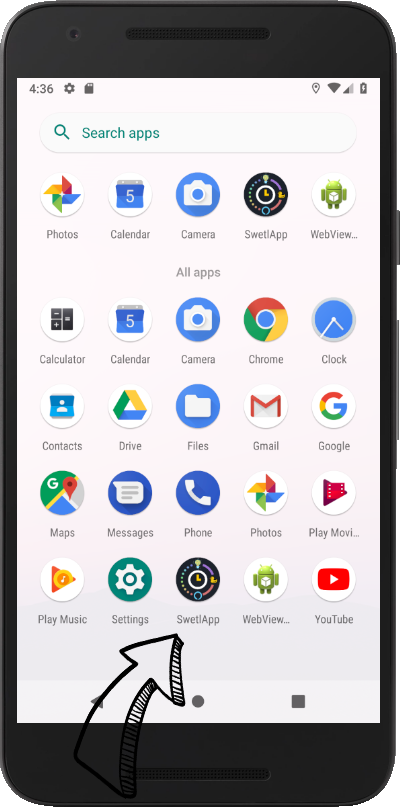
\includegraphics[width=5cm]{../includes/pics/screen1.PNG}
		\caption{\label{fig:screen1}Icona di SwetlApp su Smartphone}
	\end{figure}
	\item Ora per avviare l'applicazione basterà fare un tap sull'icona per farla eseguire.
\end{enumerate}



